
\mode<presentation>
{
  \usetheme{CambridgeUS}
  \usecolortheme{whale}
  \usecolortheme{lily}

  \setbeamercovered{transparent}
  \usefonttheme[onlymath]{serif}
}

\title[\SolvingDifferentialEquationsAndStabilityShortName] % (optional, use only with long paper titles)
{\course: \SolvingDifferentialEquationsAndStabilityName\license}

\subtitle
{Lecture \SolvingDifferentialEquationsAndStabilityNumber} % (optional)


\begin{document}

\begin{frame}
  \titlepage
\end{frame}

\mode<article>{
\maketitle
\tableofcontents
}

\section{Pre-requisite Material}
This lecture assumes that the reader is familiar with the following material:
\begin{itemize}
\item Lecture \ModelingMechanicalSystemsNumber:~\ModelingMechanicalSystemsName
\item Lecture \ElectricalSystemsNumber:~\ElectricalSystemsName
\item Lecture \LaplaceTransformReviewNumber:~\LaplaceTransformReviewName
\end{itemize}


\section{Motivation}

%\textcolor{red}{create a new introduction to this article that emphasizes the concepts: 1. we can solve diff eq's using LT. 2. more complicated Laplace domain signals can be decomposed into simpler signals that can be found in a table of LT pairs. 3. students should remember the process of finding residues to find an exact solution to the diff eq. 4. In this class, we will focus on the denominators and most often use Matlab to find the exact scaling in the numerator. 5. This will eventually bring us to the concept of stability <-- crucial topic in control systems}

In this lecture, we give a short review of differential equations, in particular solving them using Laplace Transforms. We are focused on some key concepts that help us to understand the modeling of systems (electrical, mechanical, etc.) in the Laplace domain and connecting that to what we see in the time-domain output. The block diagram below lays out the idea, 

\begin{center}
	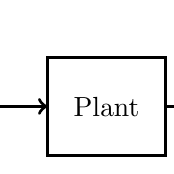
\begin{tikzpicture}[inner sep=0pt,outer sep=0pt,very thick,
sysblock/.style={draw,rectangle,inner sep=2pt,minimum width=1.5cm,minimum height=1.25cm,very thick}]
\useasboundingbox (-1,1) rectangle (0.5,-0.5); 
\begin{scope}[transform canvas={scale=1}]
\draw (0,0) node[sysblock] (S) {Plant};
\draw[->] (-2.5,0) node[above=2pt] {Input $z(t)$} -- (S.180);
\draw[->] (S.0) -- ++(2,0) node[above=2pt] {Output $y(t)$};
\end{scope}
\end{tikzpicture}

\end{center}
namely, that, 
\begin{enumerate}
	\item if we know the model of a plant system in either differential equation or transfer function\footnote{if the initial conditions are nonzero, we'll have to use the differential equation} form, and
	\item if we know the input signal $z(t)$, then
	\item we can use the Laplace transform to convert the differential equation into an algebraic relation, then
	\item solve for the Laplace transform of the solution $Y(s)$, then finally
	\item use inverse Laplace transform techniques to find the output signal $y(t)$.
\end{enumerate}

We'll use a few examples to remind you of the methods you learned in your Diff Eq class, including how to identify the form(s) of the solution to match entries in a Laplace transform pair table and how to perform partial fraction expansion (also known as partial fraction decomposition).

\section{Finding Solutions to Differential Equations}


	
%As promised, we can now solve differential equations using Laplace Transforms. 
%To solve differential equations using Laplace, we transform the differential equation into an
%algebraic relation using a Laplace Transform, solve for the Laplace
%Transform of the solution, then use inverse Laplace Transforms to bring the
%solution back into the time domain. 
The most important property of the
Laplace transform in this case is the differentiation property:%
\begin{frame}{Laplace Transform: Differentiation Property}
\begin{eqnarray*}
\mathcal{L}\left\{ \frac{d}{dt}f(t)\right\} &=&sF(s)-f(0^{-}), \\
\mathcal{L}\left\{ \frac{d^{2}}{dt^{2}}f(t)\right\} &=&s\mathcal{L}\left\{ 
\frac{d}{dt}f(t)\right\} -\frac{df}{dt}(0^{-}), \\
&=&s^{2}F(s)-sf(0^{-})-\frac{df}{dt}(0^{-}), \\
\mathcal{L}\left\{ \frac{d^{n}}{dt^{n}}f(t)\right\} &=&s^{n}F(s)-s^{n-1}f(0^{-})-
\\
&&\cdots -sf^{(n-2)}(0^{-})-f^{(n-1)}(0^{-}).
\end{eqnarray*}
\end{frame}
A good starting point to remember this is: if the initial conditions are
zero, we can replace $n^{th}$ order differentiation with $s^{n}.$ Note that
because we have defined the Laplace Transform with the lower limit of
integration zero, we must always take the starting time as $0,$ which is no
problem for linear constant coefficient differential equations.

\begin{example}
\begin{frame}
Here is a simple differential equation:%
\begin{equation*}
\frac{dy}{dt}=z(t)
\end{equation*}%
where the input $z(t)$ is the unit step function, i.e., 
\begin{equation*}
z(t) = 1\quad t\geq 0.
\end{equation*}%
What is $y(t)?$ \end{frame} Since the functions are equal on the left and right, the
Laplace Transforms will be equal: 
\begin{align*}
sY(s)-y(0^{-})&=Z(s) \\
&=\frac{1}{s}.
\end{align*}%
Solve for $Y(s):$%
\begin{equation*}
Y(s)=\frac{1}{s^{2}}+\frac{y(0^{-})}{s}.
\end{equation*}%
We recognize the Laplace Transforms on the right hand side, resulting in the solution%
\begin{equation*}
y(t)=t+y(0^{-})\quad t\geq 0.
\end{equation*}
\end{example}

\begin{example}
Let's find the position trajectory (i.e., output signal is position $x(t)$) for a mass spring damper system subject to an initial condition and an applied force (i.e., input signal is force $f(t)$).
\begin{frame}{Mass-spring-damper System}
\begin{minipage}{2.6in}
At time $t=0$, this system is at position $x=0$, but with an initial velocity of $1$ m/s. Beginning at this time, the force $f(t)=e^{-3t}$ is applied. Find $x(t)$ for $t\geq 0$.
\end{minipage}
\begin{minipage}{2in}
\begin{tikzpicture}

\draw[inner sep=0pt,outer sep=0pt,very thick] (0,-2) node[rotate=90] (gnd1) {\input{\mainfolder/DrawingElements/MechanicalElements/ground.tex}};
\draw[inner sep=0pt,outer sep=0pt,very thick] (1,0) node[rotate=90] (K1) {\begin{tikzpicture}
\draw (.75,0) node[inner sep=0,outer sep=0] (K1) {\begin{tikzpicture}
\draw (.75,0) node[inner sep=0,outer sep=0] (K1) {\input{\mainfolder/DrawingElements/MechanicalElements/spring.tex}};
\draw (K1)  node[above=6pt] {$k$};
\draw[very thick] (K1.180) -- ++(-.2,0);
\draw[very thick] (K1.0) -- ++(0.2,0);
\draw[<-,thick] (K1.0) ++(.2,0) -- ++(.5,0) node[right] {$f$};
\draw[<-,thick] (K1.180) ++(-.2,0) -- ++(-.5,0) node[left] {$f$};
\draw[|->,thick] (K1.180) ++(-.2,.4) node[above=2pt] {$x_{1}$} -- ++(.5,0);  
\draw[|->,thick] (K1.0) ++(.2,.4) node[above=2pt] {$x_{2}$} -- ++(.5,0);  
\draw<2-> (K1) ++(0,-.6) node {$f=k(x_{1}-x_{2})$};
\end{tikzpicture}
};
\draw (K1)  node[above=6pt] {$k$};
\draw[very thick] (K1.180) -- ++(-.2,0);
\draw[very thick] (K1.0) -- ++(0.2,0);
\draw[<-,thick] (K1.0) ++(.2,0) -- ++(.5,0) node[right] {$f$};
\draw[<-,thick] (K1.180) ++(-.2,0) -- ++(-.5,0) node[left] {$f$};
\draw[|->,thick] (K1.180) ++(-.2,.4) node[above=2pt] {$x_{1}$} -- ++(.5,0);  
\draw[|->,thick] (K1.0) ++(.2,.4) node[above=2pt] {$x_{2}$} -- ++(.5,0);  
\draw<2-> (K1) ++(0,-.6) node {$f=k(x_{1}-x_{2})$};
\end{tikzpicture}
};
\draw (1,0) node[right=14pt] {$2$};
\draw[inner sep=0pt,outer sep=0pt,very thick] (-1,0) node[rotate=90] (D1) {\begin{tikzpicture}
\draw[very thick] (-.2,0) -- (0,0);
\draw (.75,0) node {\begin{tikzpicture}
\draw[very thick] (-.2,0) -- (0,0);
\draw (.75,0) node {\input{\mainfolder/DrawingElements/MechanicalElements/damper.tex}};
\draw (.75,0) node[above=9pt] {$b$};
\draw[very thick] (1.5,0) -- ++(.2,0);
    \draw[<-,thick] (1.5,0) ++(.2,0) -- ++(.5,0) node[right] {$f$};
    \draw[<-,thick] (-.2,0) -- ++(-.5,0) node[left] {$f$};
    \draw[|->,thick] (-.2,.4) node[above=2pt] {$x_{1}$} -- ++(.5,0);  
    \draw[|->,thick] (1.7,.4) node[above=2pt] {$x_{2}$} -- ++(.5,0);  
    \draw (.6,-.6) node {$x=x_{1}-x_{2}$};
  %  \draw (.6,-1.2) node {$f=b\dot{x}$};
\end{tikzpicture}};
\draw (.75,0) node[above=9pt] {$b$};
\draw[very thick] (1.5,0) -- ++(.2,0);
    \draw[<-,thick] (1.5,0) ++(.2,0) -- ++(.5,0) node[right] {$f$};
    \draw[<-,thick] (-.2,0) -- ++(-.5,0) node[left] {$f$};
    \draw[|->,thick] (-.2,.4) node[above=2pt] {$x_{1}$} -- ++(.5,0);  
    \draw[|->,thick] (1.7,.4) node[above=2pt] {$x_{2}$} -- ++(.5,0);  
    \draw (.6,-.6) node {$x=x_{1}-x_{2}$};
  %  \draw (.6,-1.2) node {$f=b\dot{x}$};
\end{tikzpicture}};
\draw (-1,0) node[left=14pt] {$3$};
\draw (0,2) node[draw,rectangle,minimum width=1.5cm,minimum height=1.5cm,very thick] (M1) {$1$};

\draw[|->] (M1) ++(1.25,0) node[right] {$x$} -- ++(0,.5);

\draw[very thick] (K1.180) -- ++(0,-.25) -| (gnd1.0);
\draw[very thick] (D1.180) -- ++(0,-.25) -| (gnd1.0);
\draw[very thick] (K1.0) -- ++(0,.25) -| (M1.-90);
\draw[very thick] (D1.0) -- ++(0,.25) -| (M1.-90);
\draw[->] (M1.90)  -- ++(0,0.75) node[above] {$f(t)$};


\end{tikzpicture}
\end{minipage}
\end{frame}\vspace{.1in}

We can state this problem as solving 
\begin{equation*}
\ddot{x}+3\dot{x}+2x=e^{-3t}\qquad x(0)=0,\text{ }\dot{x}(0)=1.
\end{equation*}%
Taking the Laplace Transform of both sides:%
\begin{eqnarray*}
\left( s^{2}X(s)-1\right) +3 sX(s) +2X(s) &=&\frac{1}{s+3}, \\
\left( s^{2}+3s+2\right) X(s) &=&\frac{1}{s+3}+1 = \frac{s+4}{s+3}, \\
X(s) &=&\frac{s+4}{ (s^{2}+3s+2)(s+3) },\\
&=&\frac{s+4}{s^{3}+6s^{2}+11s+6 }.
\end{eqnarray*}%
This is the Laplace Transform of the trajectory, but what is the inverse Laplace Transform? We need to break this rational function up into parts that we can recognize by using partial fraction expansion. %This is covered in the next section.
\end{example}


\subsection{Partial Fraction Expansion}
\begin{frame}{Partial Fraction Expansion}
We can use a partial fraction expansion to break a rational function up into
easily recognizable parts that appear in a typical Laplace transform pair table. For example, we can determine from observation
that the inverse Laplace transform of 
\begin{equation*}
X(s)=\frac{3}{s-5}
\end{equation*}
is given by 
\begin{equation*}
x(t)=3e^{5t}\step(t).
\end{equation*}
\end{frame}
The partial fraction expansion method is best described using examples for some common cases, including simple real poles, complex poles, and repeated poles.

\subsubsection{Partial fraction expansion - simple real poles
\label{sec:PFEsimplePoles}}
\begin{example}
Find the inverse Laplace Transform of the output signal $X(s)$ from the mass-spring-damper example
\begin{equation*}
X(s)=\frac{s+4}{s^{3}+6s^{2}+11s+6}.
\end{equation*}

\textbf{Solution:} In order to apply the partial fraction expansion, we must
first find the roots of the denominator, which are $-1,$ $-2,$ and $-3.$ We
can rewrite $X(s)$ as 
\begin{equation*}
X(s)=\frac{s+4}{(s+1)(s+2)(s+3)}.
\end{equation*}
Since all the roots are real and simple (not multiple) we look for a partial
fraction expansion of the form 
\begin{equation*}
X(s)=\frac{A}{s+1}+\frac{B}{s+2}+\frac{C}{s+3}.
\end{equation*}
All that is left is to find the values of the unknown coefficients $A$, $B$, 
$C$, which are called \emph{residues}. There are several ways to do this:

\begin{itemize}
	\item Method 1: Equating coefficients for powers of $s$ (this section)
	\item Method 2: Finding residues directly (\ref{sec:PFErepeatedRoots})
	\item Method 3: Equating residue coefficients for selected values of $s$ (\ref{sec:PFErepeatedRoots})
\end{itemize}
Although we use different methods of finding residues to illustrate different examples in lecture and other resources, you can feel free to use whichever one(s) are most comfortable for you.
\vspace{10pt}

%\begin{description}
%\item[Method 1: Equating coefficients]  
\noindent \textbf{Method 1: Equating coefficients on powers of $s$}  
Since we need the original and expanded representations to be equal for all values of $s$, the coefficients on each power of $s$ must be equal, which gives us this first method.  
\begin{frame}{Equating Coefficients on Powers of $s$}
\begin{equation*}
\frac{s+4}{(s+1)(s+2)(s+3)}=\frac{A}{s+1}+\frac{B}{s+2}+\frac{C}{s+3}.
\end{equation*}
\end{frame}
Putting the right hand side over a common denominator, 
\begin{equation*}
\frac{s+4}{(s+1)(s+2)(s+3)}=\frac{A(s^{2}+5s+6)+B(s^{2}+4s+3)+C(s^{2}+3s+2)}{%
(s+1)(s+2)(s+3)}.
\end{equation*}
Equating coefficients gives us the three equations 
\begin{eqnarray*}
s^2: & 0 &= A+B+C, \\
s^1: & 1 &= 5A+4B+3C, \\
s^0: & 4 &= 6A+3B+2C.
\end{eqnarray*}

Solve for $A,$ $B,$and $C$ using your favorite linear algebra technique or Matlab's \texttt{rref} function:%
\begin{eqnarray*}
A &=&1.5, \\
B &=&-2, \\
C &=&0.5.
\end{eqnarray*}
so 
\begin{equation*}
X(s)=\frac{1.5}{s+1}+\frac{-2}{s+2}+\frac{0.5}{s+3}.
\end{equation*}
and we can easily find the inverse Laplace Transform, i.e., the position $x(t)$ of the mass, as
\begin{frame}{Solution to the mass-spring-damper example} 
\begin{equation*}
x(t)=(1.5e^{-t}-2e^{-2t}+0.5e^{-3t})\step(t).
\end{equation*}
What do you notice about the form of the solution to this mass-spring-damper example, given that the input force is a decaying exponential 	$f(t)=e^{-3t}$?
\begin{itemize}
	\item Does the input force pull on the mass forever or does it eventually drop to (near) zero?
	\item Does the mass eventually return to its starting position ($x(t)=0$) after enough time has passed?
	\item Do these results make sense given your understanding of masses, springs, and dampers?
\end{itemize}
\end{frame}
%\end{description}
\end{example}

%\begin{frame}
%\end{frame}
As time goes to infinity, the input force does approach 0 asymptotically, so we would expect the mass to eventually return to its neutral (unforced) position. By looking at the form of the solution $x(t)$, that is indeed what we observe for this example. 

\subsubsection{Partial fraction expansion - simple complex poles
\label{sec:PFEcomplex}}

Fundamentally, simple complex poles can be dealt with in the same way as
simple real poles. However, having complex poles can make the math more tedious when solving for the residues. Since most tables of Laplace transform pairs include cases with complex poles, it is useful to keep complex conjugate poles together and match one of the following entries in a table of Laplace transform pairs.

\begin{center}
	\begin{tabular}{| l | l | l |}
		\rule{0pt}{12pt}Function name & $f(t)$ & $F(s)$ \\ \hline
		\rule{0pt}{12pt}sine & $\sin \omega t$ & $\frac{\omega }{s^{2}+\omega ^{2}}$ \\ \hline
		\rule{0pt}{12pt}cosine & $\cos \omega t$ & $\frac{s}{s^{2}+\omega ^{2}}$ \\  \hline
		\rule{0pt}{12pt}damped sine & $e^{-at}\sin \omega t$ & $\frac{\omega }{\left( s+a\right)
			^{2}+\omega ^{2}}$ \\  \hline
		\rule{0pt}{12pt}damped cosine & $e^{-at}\cos \omega t$ & $\frac{s+a}{\left( s+a\right)
			^{2}+\omega ^{2}}$ \\  \hline
	\end{tabular}
\end{center}

As before, we'll use an example to illustrate the method.

\begin{example}
%\label{ex:PFE2}}
Find the inverse Laplace Transform of the Laplace-domain signal with \textit{complex} poles
\begin{equation*}
F(s)=\frac{3s^{2}+10s+10}{s^{3}+4s^{2}+6s+4}.
\end{equation*}

In this case, the roots of the denominator are $-2,$ $-1+j,$ $-1-j.$ We
could break this up into three terms as before, one having a real pole and the other having complex poles, but it is easier to keep the
complex conjugate poles together. Thus, the denominator can be factored as
\[
s^{3}+4s^{2}+6s+4=(s+2)(s^2+2s+2)
\]
The $2^{nd}$-order term doesn't match perfectly with any of the $F(s)$ functions in the table as currently written, but if we complete the square we see that
\[
(s^2+2s+2)=(s+1)^2+1^2,
\]
which will match one of the last two entries when $a=1$ and $\omega=1$. To finish solving the differential equation by hand, we'd need to find possible numerator values that look like (possibly scaled) $\omega$ or $s+a$ terms (and often both) according to the last two rows in the table. Our partial fraction expansion should then be structured as 
\begin{equation*}
F(s)=\frac{A}{s+2}+\frac{Bs+C}{(s+1)^2+1^2}.
\end{equation*}

At this point, we have the information we need to find the \textit{structure} of the solution, even though we don't yet know its scaling (numerator values). By comparing the expanded $F(s)$ to entries in our table of Laplace transform pairs, we can find that
\[
f(t)=\left( Ae^{-2t} + \beta e^{-t}\sin(t) + \gamma e^{-t}\cos(t) \right) u(t)
\]
where $\beta$ and $\gamma$ are finite but not-yet-known constants, and either could end up equaling zero. Here, we return to a fundamental question of control systems, namely 
\begin{frame}{Interpreting the form of the solution}
\begin{center}
\textit{Is the solution bounded or does it go to infinity as time goes to infinity}? 
\end{center}
\end{frame}

Since all of the exponential terms in $f(t)$ have negative coefficients on $t$, we can answer this question without any further math: \textit{yes, the solution is bounded, and in fact approaches zero as $t \rightarrow \infty$}. As before, this result comes from the signs on the terms in the denominator of the Laplace-domain function $F(s)$.

%The complex conjugate term must have $Bs+C$ in the numerator in order to be assured of a solution. 
For details of finding the residues $A$, $B$, and $C$ for this example please see Appendix 2. 

%\textcolor{red}{2nd lecture content starts here}

\subsection{Repeated Roots}
Since polynomials can have repeated roots, we need to determine how to take the inverse Laplace Transform when the denominator roots are repeated.

\subsubsection{Laplace Transform Pairs with repeated roots}
\begin{frame}{Laplace Transform Pairs with repeated roots}
Repeated roots occur when an exponential or sinusoid is multiplied by $t$ or $t^{n}$. First, let's derive the Laplace Transform of $t^{n}$. We already have established the Laplace Transform pair
\[
\step(t) \overset{\mathcal{L}}{\longleftrightarrow} \frac{1}{s},
\]
and the integration theorem
\[
\mathcal{L}\left\{ \int_{0}^{t}f(\tau )d\tau \right\} =%
\frac{1}{s}\mathcal{L}\left\{ f(t)\right\}. 
\]
\end{frame}
\begin{frame}{Laplace Transform Pairs with Repeated Roots}
Note that a ramp is the integral of a step. That is, the ramp function $t\step(t)$ can be defined via
\[
t\step(t) = \int_{0^{-}}^{t} \step(t) dt.
\]
Using the integration theorem gives us
\[
t\step(t) \overset{\mathcal{L}}{\longleftrightarrow} \frac{1}{s^{2}}.
\]
Thus, a ramp has two poles at $s=0$. 
\end{frame}
\begin{frame}{Higher Powers}
The Laplace Transform for higher powers of $t$ can be found via further integration. For example,
\[
\frac{1}{2}t^{2}\step(t) =  \int_{0^{-}}^{t} t\step(t) dt,
\]
which implies
\[
\frac{1}{2}t^{2}\step(t) \overset{\mathcal{L}}{\longleftrightarrow} \frac{1}{s^{3}}.
\]
and even higher orders of $t$ can be found similarly. What we see is that powers of $t$ give us a denominator with repeated roots at $s=0$. 
\end{frame}
Now, we can use the frequency shift theorem
\[
\mathcal{L}\left\{ e^{-s_{0}t}f(t)\right\}
=F(s+s_{0})
\]
to show that
\[
te^{-at} \step(t)  \overset{\mathcal{L}}{\longleftrightarrow} \frac{1}{(s+a)^{2}}.
\]
Thus the product of a ramp and exponential will give a repeated real root.

Repeated imaginary or complex roots occur when $t$ is multiplied by a sinusoid or decaying sinusoid. The following table is a partial list of the Laplace Transform pairs with repeated roots
\begin{center}
\begin{tabular}{|l|l|}
$f(t)$ & $F(s)$ \\\hline
$te^{-at}$ & $\frac{1}{(s+a)^{2}}$\\\hline
$\frac{t^{n}e^{-at}}{n!}$ & $\frac{1}{(s+a)^{n+1}}$ \\\hline
$t\sin(\omega t)$ & $\frac{2\omega s}{\left(s^{2} +\omega^{2}\right)^{2}}$ \\\hline
$te^{-at}\sin(\omega t)$ & $\frac{2\omega(s+a)}{\left((s+a)^{2} +\omega^{2}\right)^{2}}$\\\hline
\end{tabular}
\end{center}

\subsubsection{Partial Fraction Expansion with Repeated Roots
\label{sec:PFErepeatedRoots}}

Suppose we had the Laplace-domain signal
\[
X(s) = \frac{s+3}{(s^{2}+2s+1)(s+2)},
\]
and we want to find the inverse Laplace Transform. The denominator of this signal has roots at $-1, -1$ and $-2$. Thus, the root at $-1$ is repeated. In order to apply the partial fraction expansion correctly, we need one term for each root:
\[
\frac{s+3}{(s+1)^{2}(s+2)} = \frac{A}{s+1} + \frac{B}{(s+1)^{2}} + \frac{C}{s+2}
\]
Since we have expanded our Laplace Transform pairs to include repeated roots, once we find the residues, the structure of the inverse Laplace Transform is easy:
\[
x(t) = \left( A e^{-t} + B t e^{-t} + C e^{-2t} \right) u(t)
\]
and we can tell, once again, that the solution $x(t)$ will approach 0 as $t \rightarrow \infty$. (This result might not be immediately obvious due to the $t$ in the middle term, but it is outweighed by the decaying exponential.) Of course, to find the precise solution we still have to solve for the residues $A$, $B$, $C$, for which we will illustrate two methods. 
\vspace{10pt}

\noindent \textbf{Method 2: Direct Residue Formula} 

The residue formula -- a fairly direct technique -- will hold for the highest power, as well as all other terms having only non-repeated roots. In this case, the residue formula gives us
\begin{align*}
B & = \left.(s+1)^{2}\frac{s+3}{(s+1)^{2}(s+2)}\right|_{s=-1} = \frac{2}{1} = 2\\
C & = \left.(s+2)\frac{s+3}{(s+1)^{2}(s+2)}\right|_{s=-2} = \frac{1}{1} = 1
\end{align*}
However, the residue formula will {\em not} hold for $A$. There is an alternate residue formula, but it is usually easier to simply return to another method, substituting in the values for $B$ and $C$ found already. We'll illustrate our final method here:
\vspace{10pt}

\noindent \textbf{Method 3: Equating Coefficients on Residues for Selected Values of $s$}

Putting the right hand side over a common denominator.
\begin{align*}
\frac{s+3}{(s+1)^{2}(s+2)} &= \frac{A(s+1)(s+2) + 2(s+2) + 1(s+1)^2}{(s+1)^{2}(s+2)} %\\
%& = \frac{As^{2}+3As+2A + 2s+4 + s^{2}+2s+1}{(s+1)^{2}(s+2)} 
\end{align*}
Since the equality must hold for all values of $s$, we can pick one or more values to solve for any remaining residues. The choice of $s=0$ is usually convenient, as long as the denominator doesn't have a root at zero. In this case, letting $s=0$ gives us
\begin{align*}
0+3 &= A(0+1)(0+2) + 2(0+2) + 1(0+1)^2 \\
3 &= 2A + 4 + 1 \\
-2 &=2A
\end{align*}
which implies $A=-1$. If more residues remained unknown, we could pick another value of $s$ until we have as many equations as unknown.

The final partial fraction expansion becomes
\[
X(s)= \frac{-1}{s+1} + \frac{2}{(s+1)^{2}} + \frac{1}{s+2}
\]
The inverse Laplace Transform is then
\[
x(t) = \left(-e^{-t} + 2te^{-t} + e^{-2t}\right)\step(t)
\]


For higher powers, we have the general rule:

\begin{center}
\fbox{\begin{minipage}{4in}If the term $(s+a)^{n}$ appears in the denominator, then the partial fraction expansion will include the terms $(s+a)$, $(s+a)^{2}$, $\cdots$, $(s+a)^{n}$.\end{minipage}}
\end{center}

\section{Differential Equation Examples}
Let's try some examples to solidify the process of solving differential equations using Laplace Transforms.

\subsection{Example 1}
\begin{frame}{Spring and Damper}
A spring with spring constant $k=4$ N/m and damper with damping coefficient $b=2$ Ns/m is connected in parallel to a wall. A force of $f_{in}=1$ N is applied for  $t\geq0$. If the initial displacement of the right side of the spring and damper is $x=1$ m at $t=0$, find $x(t)$ for $t\geq 0$
\begin{center}
\begin{tikzpicture}[inner sep=0pt,outer sep=0pt,very thick]
\draw (1,0) node (gnd) {\input{\mainfolder/DrawingElements/MechanicalElements/ground.tex}};
\draw (3.5,0.5) node (K1) {\begin{tikzpicture}
\draw (.75,0) node[inner sep=0,outer sep=0] (K1) {\begin{tikzpicture}
\draw (.75,0) node[inner sep=0,outer sep=0] (K1) {\input{\mainfolder/DrawingElements/MechanicalElements/spring.tex}};
\draw (K1)  node[above=6pt] {$k$};
\draw[very thick] (K1.180) -- ++(-.2,0);
\draw[very thick] (K1.0) -- ++(0.2,0);
\draw[<-,thick] (K1.0) ++(.2,0) -- ++(.5,0) node[right] {$f$};
\draw[<-,thick] (K1.180) ++(-.2,0) -- ++(-.5,0) node[left] {$f$};
\draw[|->,thick] (K1.180) ++(-.2,.4) node[above=2pt] {$x_{1}$} -- ++(.5,0);  
\draw[|->,thick] (K1.0) ++(.2,.4) node[above=2pt] {$x_{2}$} -- ++(.5,0);  
\draw<2-> (K1) ++(0,-.6) node {$f=k(x_{1}-x_{2})$};
\end{tikzpicture}
};
\draw (K1)  node[above=6pt] {$k$};
\draw[very thick] (K1.180) -- ++(-.2,0);
\draw[very thick] (K1.0) -- ++(0.2,0);
\draw[<-,thick] (K1.0) ++(.2,0) -- ++(.5,0) node[right] {$f$};
\draw[<-,thick] (K1.180) ++(-.2,0) -- ++(-.5,0) node[left] {$f$};
\draw[|->,thick] (K1.180) ++(-.2,.4) node[above=2pt] {$x_{1}$} -- ++(.5,0);  
\draw[|->,thick] (K1.0) ++(.2,.4) node[above=2pt] {$x_{2}$} -- ++(.5,0);  
\draw<2-> (K1) ++(0,-.6) node {$f=k(x_{1}-x_{2})$};
\end{tikzpicture}
};
\draw (K1) node[above=14pt] {$k$};
\draw (3.5,-0.5) node (B1) {\begin{tikzpicture}
\draw[very thick] (-.2,0) -- (0,0);
\draw (.75,0) node {\begin{tikzpicture}
\draw[very thick] (-.2,0) -- (0,0);
\draw (.75,0) node {\input{\mainfolder/DrawingElements/MechanicalElements/damper.tex}};
\draw (.75,0) node[above=9pt] {$b$};
\draw[very thick] (1.5,0) -- ++(.2,0);
    \draw[<-,thick] (1.5,0) ++(.2,0) -- ++(.5,0) node[right] {$f$};
    \draw[<-,thick] (-.2,0) -- ++(-.5,0) node[left] {$f$};
    \draw[|->,thick] (-.2,.4) node[above=2pt] {$x_{1}$} -- ++(.5,0);  
    \draw[|->,thick] (1.7,.4) node[above=2pt] {$x_{2}$} -- ++(.5,0);  
    \draw (.6,-.6) node {$x=x_{1}-x_{2}$};
  %  \draw (.6,-1.2) node {$f=b\dot{x}$};
\end{tikzpicture}};
\draw (.75,0) node[above=9pt] {$b$};
\draw[very thick] (1.5,0) -- ++(.2,0);
    \draw[<-,thick] (1.5,0) ++(.2,0) -- ++(.5,0) node[right] {$f$};
    \draw[<-,thick] (-.2,0) -- ++(-.5,0) node[left] {$f$};
    \draw[|->,thick] (-.2,.4) node[above=2pt] {$x_{1}$} -- ++(.5,0);  
    \draw[|->,thick] (1.7,.4) node[above=2pt] {$x_{2}$} -- ++(.5,0);  
    \draw (.6,-.6) node {$x=x_{1}-x_{2}$};
  %  \draw (.6,-1.2) node {$f=b\dot{x}$};
\end{tikzpicture}};
\draw (B1) node[below=14pt] {$b$};


\draw (K1.180) -- (K1.180 -| gnd.0);
\draw (B1.180) -- (B1.180 -| gnd.0);
\draw (K1.0) -- ++(0.5,0) |- ++(1,-.5) node[circle,fill,inner sep=0] (F) {\rule{0pt}{4pt}};
\draw (B1.0) -- ++(0.5,0) |- ++(0,.5);
\draw[|->,thick] (F) ++(0,.5) node[above=6pt] {$x$} -- ++(.5,0);
\draw[->,thick] (F) -- ++(.75,0) node[right=2pt] {$f_{in}$}; 

\end{tikzpicture}
\end{center}
\end{frame}
This system is governed by the differential equation
\[
b \dot{x} + k x = f_{in}  \\
\]
Thus, we can ask: what is the solution to the differential equation
\[
2 \dot{x} + 4 x = 1 \qquad x(0)=1 \\
\]
\tryit{
\begin{boxedminipage}{6.5 in}
\rule{0pt}{12pt}\vspace{2in}
\color{lightgray}
\[
x(t) = \left(\frac{1}{4} + \frac{3}{4}e^{-2t}\right)\step(t)
\]
\end{boxedminipage}\\
}{\begin{boxedminipage}{6.5in}
Take the Laplace Transform of both sides:
\[
2(sX(s) - 1) + 4X(s) = \frac{1}{s}
\]
Solve for X(s):
\begin{align*}
(2s+4)X(s) &= \frac{2s+1}{s} \\
X(s) = \frac{s +\frac{1}{2} }{s(s+2)}
\end{align*}
Find partial fraction expansion:
\begin{align*}
\frac{s +\frac{1}{2} }{s(s+2)} = \frac{A}{s} + \frac{B}{s+2}
\end{align*}
where
\begin{align*}
A &= \left.\frac{s +\frac{1}{2} }{s+2}\right|_{s=0} = \frac{1}{4}\\
B &= \left.\frac{s +\frac{1}{2}}{s}\right|_{s=-2} = \frac{3}{4}\\
\end{align*}
Giving inverse Laplace Transform
\[
x(t) = \left(\frac{1}{4} + \frac{3}{4}e^{-2t}\right)\step(t)
\]
\end{boxedminipage}
}

Notice that in this mass-spring-damper example, there is a constant, nonzero force applied as the input signal $f_{in}$. As a result, the mass does not return to its initial position as $t \rightarrow \infty$, but it does approach a constant, bounded value $\left( \frac{1}{4} \right)$. 

\subsection{Example 2}
\begin{frame}{Circuit Problem}
\begin{center}
An LRC circuit has applied voltage $v_{in}=1$ for $t\geq0$. If $v_{out}(t)$ was zero for $t\leq0$, find $v_{out}(t)$ for $t\geq 0$.\\
\input{figures/seriescircuit.tex}
\end{center}
\end{frame}

Previously, we found that this system was governed by the differential equation
\[
CL\ddot{v}_{out}+CR\dot{v}_{out} + v_{out} = v_{in}
\]
Thus, we can ask: what is the solution to the differential equation
\begin{equation*}
\frac{1}{4}\ddot{v}_{out}+\dot{v}_{out}+v_{out}=1\qquad v_{out}(0)=0,\text{ }\dot{v}_{out}(0)=0
\end{equation*}%
\tryit{
\begin{boxedminipage}{6.5 in}
\rule{0pt}{12pt}\vspace{2in}
\color{lightgray}
\[
v_{out}(t) = (1 - e^{-2t} -2te^{-2t})\step(t)
\]
\end{boxedminipage}\\
}{\begin{boxedminipage}{6.5in}
First, take the Laplace Transform of both sides (noting that initial conditions are zero):
\[
\frac{1}{4}s^{2}V_{out}(s) + sV_{out}(s) + V_{out}(s) = \frac{1}{s}.
\]
Then, solve for $V_{out}(s):$
\begin{align*}
V_{out}(s) &= \frac{4}{(s^{2}+4s+4)s} \\
&= \frac{4}{s(s+2)^{2}} \\
\end{align*}
Find partial fraction expansion:
\[
V_{out}(s) = \frac{A}{s} +\frac{B}{s+2} + \frac{C}{(s+2)^{2}}
\]
Residues:
\begin{align*}
A &= \left.\frac{4}{(s+2)^{2}}\right|_{s=0} = 1\\
C & =\left.\frac{4}{s}\right|_{s=-2} = -2 
\end{align*}
Solve for remaining coefficients
\[
\frac{4}{s(s+2)^{2}} = \frac{(s^{2}+4s+4) + B(s^{2}+2s) - 2s}{s(s+2)^{2}} 
\]
Thus $B=-1$, and
\[
v_{out}(t) = (1 - e^{-2t} -2te^{-2t})\step(t)
\]
\end{boxedminipage}}

Similarly to the mass-spring-damper example, the input signal for this circuit example is a nonzero constant for all $t \geq 0$. As the solution shows, this also results in a constant, nonzero value for the output signal $v_{out}$. These results bring us to one of the most important concepts in control theory: stability. 

\section{Stability}
\begin{frame}{Definition of BIBO Stability}
\begin{definition}
	A system is {\em Bounded Input Bounded Output} (BIBO) {\em stable} if every bounded input results in a bounded output
\end{definition}

How does this definition relate to the concepts in this lecture?
\end{frame}

In this lecture, you have seen the idea behind stability several times when noticing whether certain signals converge to a constant value, remain bounded (e.g., a $\sin$ wave with constant amplitude), or diverge (approach infinity in magnitude). 

However, it's important to realize that all of the examples in this lecture are calculated \textit{only for a specific input signal}, whereas the definition of BIBO stability requires the output signal to remain bounded for \textit{all possible bounded input signals}. In other words, you can \textit{disprove} stability by finding a single bounded input that results in an unbounded output, but you cannot \textit{prove} stability by showing that the output signal is bounded for one selected input signal like those in this article. We'll thus be returning to this concept frequently in the coming lectures. 

%\begin{definition}
%	A rational transfer function $G(s)$ is {\em proper} if the number of poles is greater than or equal to the number of zeros 
%\end{definition}
%
%\begin{fact}
%	An LTI system with transfer function $G(s)$ is BIBO stable if and only if $G(s)$ is proper and all poles $p_{i}$ satisfy $\mbox{Re}\{p_{i}\}<0$.
%\end{fact}
%
%\begin{frame}{BIBO Stability Examples}
%\begin{center}
%	\begin{tikzpicture}
\draw (0,1.75) node {BIBO stable};
\draw (0,0) node {
\begin{tikzpicture}[scale=.4]
\draw[->] (-6,0) -- (2,0) node[below=2pt] {Re$(s)$};
\draw[->] (0,-3) -- (0,3) node[left=2pt] {Im$(s)$};
\draw (-4,0) node {\Large\sf x};
\draw (-1,1) node {\Large\sf x};
\draw (-1,-1) node {\Large\sf x};
\end{tikzpicture}};

\draw (5,1.75) node {not BIBO stable};
\draw (5,0) node {
\begin{tikzpicture}[scale=.4]
\draw[->] (-6,0) -- (2,0) node[below=2pt] {Re$(s)$};
\draw[->] (0,-3) -- (0,3) node[left=2pt] {Im$(s)$};
\draw (1,0) node {\Large\sf x};
\draw (-1,1) node {\Large\sf x};
\draw (-1,-1) node {\Large\sf x};
\end{tikzpicture}};

\draw (2.5,-1.75) node {not BIBO stable};
\draw (2.5,-3.5) node {
\begin{tikzpicture}[scale=.4]
\draw[->] (-6,0) -- (2,0) node[below=2pt] {Re$(s)$};
\draw[->] (0,-3) -- (0,3) node[left=2pt] {Im$(s)$};
\draw (-4,0) node {\Large\sf x};
\draw (0,1) node {\Large\sf x};
\draw (0,-1) node {\Large\sf x};
\end{tikzpicture}};



\end{tikzpicture}
%\end{center}
%\end{frame}


%\section{Application Example \textcolor{red}{consider removing for length, or maybe incorporate into stability discussion?}} %new


\section{Lecture Highlights}
The primary takeaways from this article include
\begin{enumerate}
\setlength{\itemsep}{5pt}
\setlength{\parskip}{0pt}
\setlength{\parsep}{0pt}
\item The Laplace transform and inverse Laplace transform can be used to solve differential equations.
\item The differentiation property of the Laplace transform is the most important property to know for this class.
\item Set up partial fractions such that each fraction is consistent with a Laplace transform pair from an available table of pairs. 
\item When the Laplace domain function has repeated roots in the denominator, the structure of the partial fraction expansion requires a term for each root.
\item If there are repeated roots in the Laplace domain, you will find the multiplier $t$ in your time domain solution.
\item The three primary methods for solving for the coefficients $A$, $B$, $C$, etc. in your partial fraction expansion are (1) equating coefficients for each power of $s$, (2) finding residuals directly, and (3) equating coefficients for selected values of $s$.
\item After you have solved for the coefficients, use the Laplace transform pair table to convert to the time-domain solution of the differential equation.
\item The concept of stability is one of the most important in control theory. In this lecture, you've seen the idea of the concept introduced by evaluating whether a signal diverges as time $t \rightarrow \infty$, but \textit{convergence of an output signal for a single input signal is not sufficient to prove stability.} We'll be returning to the concept in the coming lectures. 
\end{enumerate}

\section{Quiz Yourself}

\subsection{Questions}


\begin{enumerate}
\setlength{\itemsep}{5pt}
\setlength{\parskip}{0pt}
\setlength{\parsep}{0pt}
\item Find the Inverse Laplace Transform of the following functions
\begin{enumerate}
\setlength{\itemsep}{5pt}
\setlength{\parskip}{0pt}
\setlength{\parsep}{0pt}
\item $F(s) = \frac{3s+1}{s(s+1)(s+2)}$
\item $F(s) = \frac{3s+1}{s(s^{2}+4s+4)}$
\end{enumerate}

\item A motor on a car can be considered an input force for the car
\begin{enumerate}
	\item Find a differential equation relating the input force and the velocity of the car. Include the mass of the car and viscous friction (air and rolling resistance.) Assume the car is on level ground.
	\item Assume that the velocity of the car is 40 m/s and the car starts to coast at $t=0$. Find the velocity $v(t)$ for $t\geq 0$ if the mass of the car is $1000$ kg and the viscous friction is $125$ N sec/m.  
	\item Determine how long it will take the car to slow to $5 m/s$.
	\item Sketch the output as a function of time.
\end{enumerate}

%\item \input{quizfigures/prostheticQYproblem.tex}
\item \input{quizfigures/windQYproblem.tex}

\end{enumerate}

\subsection{Solutions}
\begin{enumerate}
\setlength{\itemsep}{5pt}
\setlength{\parskip}{0pt}
\setlength{\parsep}{0pt}
\item \rule{0pt}{12pt}\\
\begin{enumerate}
\setlength{\itemsep}{5pt}
\setlength{\parskip}{0pt}
\setlength{\parsep}{0pt}
\item \rule{0pt}{12pt}\\
\begin{center}
\includegraphics[width=4in]{quizfigures/1asoln}
\end{center}
\item \rule{0pt}{12pt}\\
\begin{center}
\includegraphics[width=4in]{quizfigures/1bsoln}
\end{center}
\end{enumerate}

\item \rule{0pt}{12pt}\\
\begin{enumerate}
	\setlength{\itemsep}{5pt}
	\setlength{\parskip}{0pt}
	\setlength{\parsep}{0pt}
	\item \rule{0pt}{12pt}\\
	\begin{center}
		\includegraphics[width=3in]{quizfigures/3asoln}
	\end{center}
	\item \rule{0pt}{12pt}\\
	\begin{center}
		\includegraphics[width=3in]{quizfigures/3bsoln}
	\end{center}
	\item \rule{0pt}{12pt}\\
	\begin{center}
		\includegraphics[width=3in]{quizfigures/3csoln}
	\end{center}
	\item \rule{0pt}{12pt}\\
	\begin{center}
		\includegraphics[width=3in]{quizfigures/3dsoln}
	\end{center}
\end{enumerate}

%\item \input{quizfigures/prostheticQYsoln.tex}
\item \input{quizfigures/windQYsoln.tex}

\end{enumerate}

\section{Resources}

\subsection{Books}
Solving linear differential equations is one of the principle uses of the Laplace Transform, and is covered in introductory controls and advanced engineering math textbooks.

\begin{itemize}
\item Gene F. Franklin, J. David Powell and Abbas Emami-Naeini,  {\em Feedback Control of Dynamic Systems}, Pearson
\begin{itemize}
\item 6th and 7th edition: Section 3.1.7
\end{itemize}
\item Erwin Kreyszig, {\em Advanced Engineering Mathematics}, Wiley
\begin{itemize}
\item 10th edition: Section 6.2
\end{itemize}
\end{itemize}

\subsection{Web resources}
There are also some web resources that cover solving differential equations using Laplace Transforms. If you find something useful, or if you find a link that no longer works, please inform your instructor!


\begin{itemize}
\item From the Khan Academy some videos on  \href{https://www.khanacademy.org/math/differential-equations/laplace-transform/laplace-transform-to-solve-differential-equation/v/laplace-transform-to-solve-an-equation}{solving differential equations}. 
\end{itemize}

\section{Appendix 1: Laplace Transform Table}

Here is a summary of the Laplace Transforms and other results derived in the last few lectures. 

\begin{center}
\resizebox{5in}{!}{\begin{tabular}{cc}\toprule
\multicolumn{2}{c}{Laplace transform pairs}\\\midrule
\hspace{1in}$f(t)$\hspace{1in} & \hspace{1in}$F(s)$\hspace{1in}  \\\midrule
\rule{0pt}{16pt}Unit impulse $\delta(t)$ & 1 \\[.15cm]\midrule
\rule{0pt}{16pt}Unit step $\step(t)$ & $\frac{1}{s}$ \\[.15cm]\midrule
\rule{0pt}{16pt}$t\step(t)$ & $\frac{1}{s^2}$ \\[.15cm]\midrule
\rule{0pt}{16pt}$\frac{1}{2}t^{2}\step(t)$ & $\frac{1}{s^{3}}$  \\[.15cm]\midrule
\rule{0pt}{16pt}$Ae^{at}\step(t)$ & $\frac{A}{s-a}$  \\[.15cm]\midrule
\rule{0pt}{16pt}$te^{at}\step(t)$ & $\frac{1}{(s-a)^{2}}$ \\[.15cm]\midrule
\rule{0pt}{16pt}$\frac{1}{2}t^2e^{at}\step(t)$ & $\frac{1}{(s-a)^{3}}$ \\[.15cm]\midrule
\rule{0pt}{16pt}$\sin(\omega t)\step(t)$ & $\frac{\omega}{s^2+\omega^2}$ \\[.15cm]\midrule
\rule{0pt}{16pt}$\cos(\omega t)\step(t)$ & $\frac{s}{s^2 + \omega^2}$ \\[.15cm]\midrule
\rule{0pt}{16pt}$e^{-at}\sin(\omega t)\step(t)$ & $\frac{\omega}{(s+a)^2+\omega^{2}}$ \\[.15cm]\midrule
\rule{0pt}{16pt}$e^{-at}\cos(\omega t)\step(t)$ & $\frac{s+a}{(s+a)^2+\omega^{2}}$ \\[.15cm]\midrule
\rule{0pt}{16pt}$\frac{df}{dt}$  & $sF(s) - f(0^{-})$ \\[.15cm]\midrule
\rule{0pt}{16pt}$\frac{d^{n}f}{dt^{n}}$ & $s^{n}F(s) - \sum_{k=1}^{n}s^{n-k}\frac{d^{k-1}f}{dt^{k-1}}(0^{-})$ \\[.15cm]\midrule
\rule{0pt}{16pt}$\int_{0}^{t} f(\tau)d\tau$ & $\frac{F(s)}{s}$ \\[.15cm]
\bottomrule
\end{tabular}}\vspace{.1in}
\end{center}



%\section{Appendix 1: Residue Formula}
%\noindent \textbf{Finding Residues Method 3: Finding residues directly}  
%Consider again the problem of finding the coefficients in Example textcolor{red}{figure out how to auto-reference an example}. We again start with the
%fundamental desired equality 
%%\begin{frame}{Finding Residues Directly} % frame was for when included in article
%\begin{equation*}
%X(s)=\frac{s+4}{(s+1)(s+2)(s+3)}=\frac{A}{s+1}+\frac{B}{s+2}+\frac{C}{s+3}.
%\end{equation*}
%%\end{frame}
%Now, if we multiply both sides by $(s+1)$, we get 
%\begin{equation*}
%(s+1)X(s)=\frac{s+4}{(s+2)(s+3)}=A+\frac{(s+1)B}{s+2}+\frac{(s+1)C}{s+3}.
%\end{equation*}
%Letting $s=-1,$%
%\begin{equation*}
%\left. (s+1)X(s)\right| _{s=-1}=\frac{3}{1\cdot 2}=A+0+0.
%\end{equation*}
%We have found an equation for $A!$ Clearly, $A=1.5,$ as we saw before. In
%general, to find the residue of a simple pole $p_{i}$, multiply the rational
%function by $(s-p_{i})$ and let $s=p_{i},$ the result is the residue. We
%find 
%\begin{eqnarray*}
%B &=&\left. (s+2)X(s)\right| _{s=-2}=\frac{2}{(-1)(1)}=-2, \\
%C &=&\left. (s+3)X(s)\right| _{s=-3}=\frac{1}{(-2)(-1)}=0.5.
%\end{eqnarray*}
%as expected.
 
\mode<article>{
\section{Appendix 2: Finding Residues for the Example in Section \ref{sec:PFEcomplex}}
We'll find the residues to complete the example using residue calculation methods for further illustration. We can find $A$ quickly using the direct residue method (Method 2): 
\begin{equation*}
A=\left. (s+2)F(s)\right| _{s=-2}=\left. \frac{3s^{2}+10s+10}{(s+1)^2+1^2}%
\right| _{s=-2}=\frac{12-20+10}{1+1}=\frac{2}{2}=1,
\end{equation*}
while $B$ and $C$ can be found by equating coefficients on the residues for convenient values of $s$.

So far, we have
\begin{equation*}
F(s)=\frac{3s^{2}+10s+10}{s^{3}+4s^{2}+6s+4}=\frac{1}{s+2}+\frac{Bs+C}{(s+1)^2+1^2}.
\end{equation*}
Since there is no denominator root at zero, let's start with $s=0$. We get
\begin{eqnarray*}
	\frac{3\left( 0\right) ^{2}+10\left( 0\right) +10}{\left( 0\right)
		^{3}+4\left( 0\right) ^{2}+6\left( 0\right) +4} &=&\frac{1}{0+2}+\frac{%
		B\left( 0\right) +C}{\left( 0 + 1 \right) ^{2} + 1^2}, \\
	\frac{10}{4} &=&\frac{1}{2}+\frac{C}{2}, \\
	4 &=&C,
\end{eqnarray*}
giving us $C$ directly. Picking another reasonably convenient value $s=1$ and plugging it into both sides, we get 
\begin{eqnarray*}
	\frac{3\left( 1\right) ^{2}+10\left( 1\right) +10}{\left( 1\right)
		^{3}+4\left( 1\right) ^{2}+6\left( 1\right) +4} &=&\frac{1}{1+2}+\frac{%
		B\left( 1\right) +C}{\left( 1+1 \right) ^{2} + 1^2}, \\
	\frac{23}{15} &=&\frac{1}{3}+\frac{B+C}{5}, \\
	6 &=&B+C,
\end{eqnarray*}
or $B=6-4=2.$
%\end{description}

This gives us 
\begin{equation*}
F(s)=\frac{1}{s+2}+\frac{2s+4}{ \left( s+1 \right) ^2 + 1^2}.
\end{equation*}
The final step is to find the inverse Laplace Transform. The first term is
easy, as we recognize it as an exponential. For the second term, 
%we need to look at the transform pairs that involve complex conjugate roots:
%
%First, we should put the denominator into the form $(s+a)^{2}+\omega ^{2}$
%by completing the square 
%\begin{eqnarray*}
%s^{2}+2s+2 &=&s^{2}+2s+1+1, \\
%&=&\left( s+1\right) ^{2}+1.
%\end{eqnarray*}
%Then, 
we need to put the numerator into the correct form, 
\begin{equation*}
2s+4=2(s+1)+2
\end{equation*}
so we have 
\begin{equation*}
\frac{2s+4}{(s+1)^{2}+1}=2\frac{(s+1)}{(s+1)^{2}+1}+2\frac{1}{(s+1)^{2}+1},
\end{equation*}
or 
\begin{equation*}
F(s)=\frac{1}{s+2}+2\frac{(s+1)}{(s+1)^{2}+1}+2\frac{1}{(s+1)^{2}+1},
\end{equation*}
i.e., our previously unknown constants $\beta=2$ and $\gamma=2$ and 
\begin{equation*}
f(t)=(e^{-2t}+2e^{-t}\cos (t)+2e^{-t}\sin (t))\step(t),
\end{equation*}
by inspection.
\end{example}
}

\end{document}


